%! TEX rootmain.tex

\chapter{Mallet Percussion Instruments}

Mallet percussion instruments belong to the family of idiophones, where the sound is produced by the vibration of the instrument body itself. In the tuned members of this family, pitch perception is shaped by the inharmonic modal structure of bars or rods and, when present, by auxiliary resonators that increase radiation efficiency and loudness. The chapter introduces a basic taxonomy of idiophones and then focuses on bar-based mallet instruments, discussing typical construction choices, overtone-tuning strategies, and the role of the mallet in controlling excitation bandwidth. The discussion is organized as follows:

\begin{itemize}
  \item idiophones and a basic classification into tuned and untuned instruments
  \item general features of mallet percussion instruments based on free bars or rods
  \item selected tuned bar instruments: glockenspiel, marimba, xylophone, and vibraphone
  \item the role of mallets in controlling spectral content through contact mechanics
\end{itemize}

\section{Idiophones}

Idiophones are instruments in which the sound is generated by the vibration of the whole object, without relying on dedicated vibrating elements such as strings or membranes. Depending on the instrument, vibration may be initiated by plucking, rubbing, or striking. Idiophones are commonly subdivided into one-dimensional and two-dimensional families, according to whether the dominant vibrating element behaves mainly like a bar/rod or like a plate. A further practical distinction is between tuned and untuned idiophones. Typical examples include:

\begin{itemize}
  \item tuned idiophones, such as xylophones, marimbas, vibraphones, bells, agogo and handpans,
  \item untuned idiophones, such as cymbals, tam-tams, triangles, and woodblocks.
\end{itemize}

\section{Mallet Percussion Instrument Characteristics}

A mallet percussion instrument is typically built as a collection of thin bars or rods with free ends. Each bar or rod behaves as a one-dimensional idiophone and is set into vibration by striking it with dedicated sticks called mallets. Because the flexural modes of free bars are not harmonically related, such instruments naturally exhibit an inharmonic overtone progression. For this reason, overtone tuning is often used to reshape selected modal frequencies so that the radiated spectrum supports a clearer pitch impression. When bars share the same geometry and size, the material plays a primary role in setting modal frequencies. The relevant elastic properties, and therefore stiffness, influence the characteristic velocity of mechanical-wave propagation in the bar, which in turn affects the modal frequencies set.

\section{Glockenspiel}

The glockenspiel uses rectangular steel bars, typically \SIrange{2.5}{3.2}{\centi\meter} wide and \SIrange{6}{9}{\milli\meter} thick. Its common range spans from G5 (\SI{784}{\hertz}) up to C8 (\SI{4186}{\hertz}). It is played with brass or plastic mallets. In this instrument, higher partials decay quickly and lie in a very high-frequency region, where pitch discrimination is reduced. As a consequence, little or no overtone tuning is typically pursued, and the sound rapidly settles to a recognizable pitch impression.

\subsection{Main Vibrational Modes}

Mode-shape diagrams (reported in figure \ref{fig:glockenspielmode}) commonly highlight a longitudinal mode and transverse modes in the plane of the bar (often indicated as the first and second transverse families). These families coexist and may contribute differently depending on the excitation point and mallet characteristics. 

\begin{figure}[!htb]
    \centering
    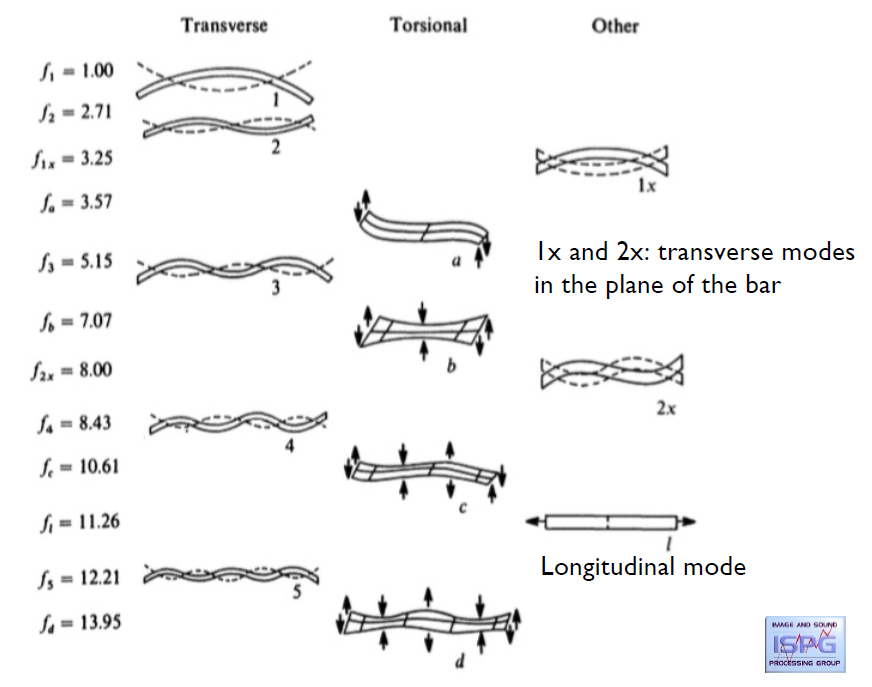
\includegraphics[width=0.7\linewidth]{00_Images/08,09,10_chapter/03.png}
    \caption{Glockenspiel main vibrational modes}
    \label{fig:glockenspielmode}
\end{figure}

\section{Marimba}

The marimba uses rectangular rosewood bars, typically \SIrange{4.5}{6.4}{\centi\meter} wide, arranged to cover about 3 to 4.5 octaves (often from A2 to C7, depending on the model). Under each bar, resonant tubes are positioned and tuned to the pitch of the corresponding bar. Unlike a simple rectangular section, marimba bars are shaped with an arched profile. This profile is a core design choice for both pitch range and spectral control.

\subsection{Marimba bars shape}

A section view of a marimba bar reveals the arched shape. This shaping serves two purposes: it allows lower pitches to be reached for a given bar length, and it enables overtone tuning. A common target is to tune the first overtone approximately two octaves above the fundamental, corresponding to a frequency ratio of about \( 4 \) relative to the fundamental. The associated mode-shape sketches typically show the transverse families for a tuned bar and the corresponding material-removal profile. A concise comparison between the modal shapes of standard rectangular bars and marimba bars is shown in figure \ref{fig:comparison}, highlighting how the location of displacement maxima shifts from the ends to the center and directly affects the optimal striking position for emphasizing specific overtones.

\begin{figure}[!htb]
    \centering
    \subfloat[Standard rectangula bar]{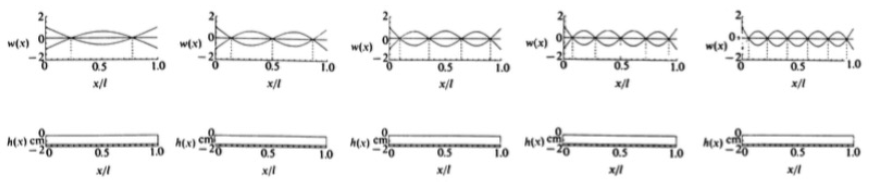
\includegraphics[width=0.7\linewidth]{00_Images/08,09,10_chapter/04_1.png}}\\
    \subfloat[Marimba bar]{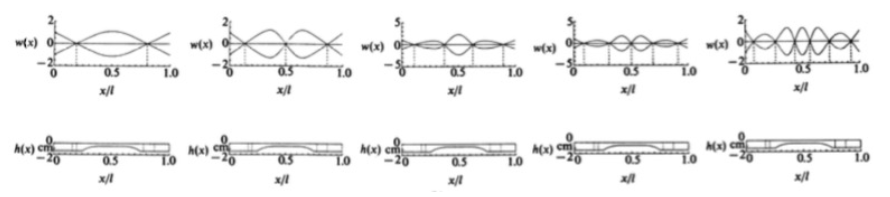
\includegraphics[width=0.7\linewidth]{00_Images/08,09,10_chapter/04_2.png}}\\
    \caption{Comparison between the modal shapes of standard rectangular bars and marimba bars}
    \label{fig:comparison}
\end{figure}

\paragraph{Where to Strike} A standard rectangular bar tends to have displacement maxima near the ends, whereas marimba bars are designed so that the displacement maximum occurs near the center. This matters for performance practice: the striking point can be chosen to emphasize or suppress specific overtones, depending on how strongly the impact couples into each modal shape.

\subsection{Tuning Procedures}

Material removal at selected points can be used to target individual modal frequencies. Removing material in regions where the bending moment of a given mode is large tends to lower the frequency of that mode significantly. Conversely, to raise the overall modal frequencies, material removal should be applied near the endpoints of the bar.

\subsection{Resonators}

Cylindrical pipe resonators, often closed at one end, are placed under each bar to emphasize the bar tone. The tube length is tuned to correspond to one quarter of the wavelength of the target bar tone, i.e., a quarter-wave relationship. The presence of resonators increases loudness while shortening decay time. In some listening conditions, this faster decay may still be perceived as a longer-lasting sound because the increased loudness remains above the ambient noise floor for longer. From a radiation viewpoint, the resonator increases acoustic efficiency by rephasing the field so that a dipole-like radiating bar behaves more like a monopole. This explains why the sound is louder and why energy is radiated away more efficiently, leading to faster decay. Closed-end resonators emphasize odd harmonics, so the resonator effect primarily influences the corresponding odd components of the bar spectrum. Even harmonics above the second are less affected. The distance between the bar and the resonator opening also matters because it affects the standing-wave pattern in the tube; in some designs, this distance can be adjusted to gently lower or raise tube resonances. A sketched representation of the sound decay with (line A) and without (line B) the resonators is reported in figure \ref{fig:decay}.

\begin{figure}[!htb]
    \centering
    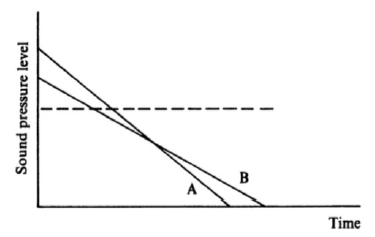
\includegraphics[width=0.5\linewidth]{00_Images/08,09,10_chapter/05.png}
    \caption{Sound decay with (line A) and without (line B) the resonators}
    \label{fig:decay}
\end{figure}

\section{Xylophone}

Modern xylophones are structurally similar to marimbas. A common difference is the absence of resonators, although some instruments may include them. The bars are often shaped underneath to manipulate overtone relationships. The overall sound character differs significantly: marimbas are typically duller and rounder, while xylophones are more brilliant and cutting. A typical tuning goal is to set the first overtone near three times the fundamental frequency, reinforcing a brighter, more incisive spectral profile.

\section{Vibraphone}

The vibraphone uses aluminum bars that are deeply arched, so the first harmonic occurs at approximately four times the fundamental frequency. Since aluminum decays more slowly than wood, a pedal-controlled damping mechanism is included, often implemented with a felt damper under the bars. A defining feature is the use of a mechanical motor to produce a vibrato-like effect, which motivates the instrument name.

\subsection{Motor-Driven Resonator Modulation}

Motor-driven disks on the resonators cyclically open and close the tubes. This periodic modulation produces an amplitude vibrato effect. Decay-rate plots typically show how the sustained tone is shaped over time in the presence of this modulation. A sketched representation of the sound decay is reported in figure \ref{fig:decayvibra}.

\begin{figure}[!htb]
    \centering
    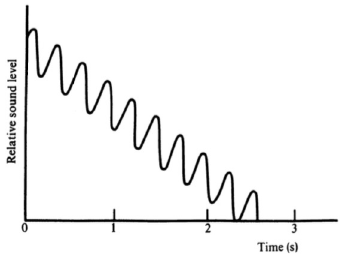
\includegraphics[width=0.5\linewidth]{00_Images/08,09,10_chapter/06.png}
    \caption{Sound decay of a vibraphone}
    \label{fig:decayvibra}
\end{figure}

\section{Mallets}

A wide variety of mallets exists, and mallet characteristics strongly influence the timbre by changing how energy is delivered to the bar and which frequency regions are excited. Three key parameters are typically emphasized:

\begin{itemize}
  \item hardness, since harder mallets more readily excite higher overtones, while softer mallets yield a rounder sound
  \item mass, which contributes to the energy transferred and, through inertia, affects contact time; longer contact times tend to damp higher partials more strongly
  \item impact velocity, which also affects contact time and mallet deformation; increased deformation can raise effective stiffness during contact and influence the highest harmonic efficiently excited
\end{itemize}

Figure \ref{fig:mallet} reports plots comparing different mallets report the maximum frequency effectively solicited as a function of impact velocity for mallets of different hardness, illustrating how the excitation bandwidth evolves with playing intensity.

\begin{figure}[!htb]
    \centering
    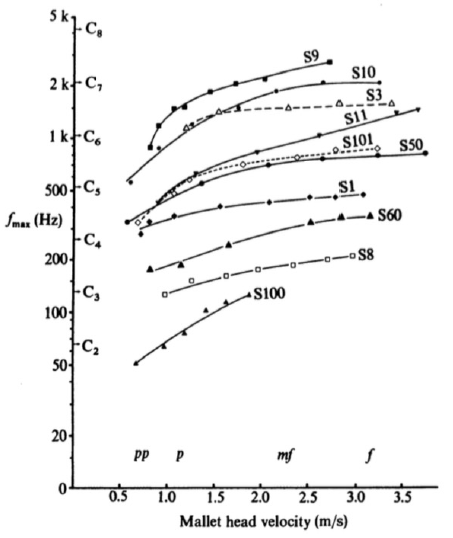
\includegraphics[height=0.3\textheight]{00_Images/08,09,10_chapter/07.png}
    \caption{Comparison between different mallets}
    \label{fig:mallet}
\end{figure}